\documentclass[conference]{IEEEtran}
\IEEEoverridecommandlockouts
% The preceding line is only needed to identify funding in the first footnote. If that is unneeded, please comment it out.
\usepackage{cite}
\usepackage{amsmath,amssymb,amsfonts}
%\usepackage{algorithmic}
%TODO: Darf man das nutzen bei IEEE?
\usepackage{mathtools}
\usepackage{comment}
\usepackage{graphicx}
\usepackage{textcomp}
\usepackage{acronym}
\usepackage{url}
\usepackage{float}
\usepackage{amsmath}
\usepackage{diagbox}
\usepackage{amssymb}
\usepackage{enumitem}
\newcommand{\code}[1]{\texttt{#1}}
\usepackage[ruled,vlined,linesnumbered]{algorithm2e}

% custom macros used in algorithms
\newcommand{\var}[1]{#1}
\newcommand{\func}[1]{\texttt{#1}}

\usepackage{xcolor}
\usepackage[hidelinks]{hyperref} % load last
\Urlmuskip=0mu plus 1mu\relax
\def\UrlBreaks{\do\/\do-\do\_}
\def\BibTeX{{\rm B\kern-.05em{\sc i\kern-.025em b}\kern-.08em
    T\kern-.1667em\lower.7ex\hbox{E}\kern-.125emX}}


\pdfobjcompresslevel=0
\pdfminorversion=4
\hypersetup{pdfcreator={}, pdfproducer={}}
    
\begin{document}

\title{Adaptive Offloading
of Scientific Workflow Jobs
Across Multi-Cluster Environments}

\author{
    %\IEEEauthorblockN{\IEEEauthorrefmark{1}, \IEEEauthorrefmark{1}, \IEEEauthorrefmark{1},}

    \IEEEauthorblockA{
    Anonymous Authors
        %\{firstname.lastname\}@tu-berlin.de, Technische Universität Berlin, Germany\\
    }


}

%\IEEEpubid{\makebox[\columnwidth]{*equal contribution, alphabetical order \hfill} \hspace{\columnsep}\makebox[\columnwidth]{ }}

\maketitle

\begin{abstract}
Scientific workflows orchestrate complex data analyses on large, compute-intensive datasets that often exceed the capacity of a single computer or even a single cluster.
Offloading jobs across multiple clusters can alleviate resource constraints and shorten execution time while controlling cost. 

This paper proposes adaptive offloading of workflow jobs in multi-cluster environments to meet user-defined makespan deadlines while minimizing execution costs. 
We propose a heuristic based on a two-step prediction approach: (i) predicting individual job runtimes using a regression model trained on historical executions and (ii) simulating workflow execution to estimate makespan and cost for alternative offloading configurations.

The method is implemented as an extension of the Snakemake workflow management system and is evaluated with three real-world bioinformatic workflows. 
By determining the locally optimal subset of jobs to offload, our approach reduces the overall workflow makespan by up to 36.51\% compared to a single-cluster baseline and reduces costs under deadline constraints by approximately 52\% compared to naive offloading, while maintaining absolute makespan prediction errors between 0.21\% and 16.88\%.

\end{abstract}

% from other papers
% Energy measurement, Supercomputers, Microprocessors, Multicore processing, Load modeling, High performance computing, Cluster computing, Power measurement, Software evaluation, Experimental comparison, DC power consumption, processor power, power model, multicore processor, processor workload analysis, processor power consumption estimation

% TODO: Refine
\begin{IEEEkeywords}
Job Offloading, Scientific Workflow, Cloud Computing, Machine Learning, Deadline Constraint, Cost Optimization
\end{IEEEkeywords}

\section{Introduction} % 1/2 Seite
\label{sec:introduction}
Data-driven science has produced massive datasets from high-throughput instruments, large simulations, and pervasive sensing \cite{noauthororeditorfourth, liew_scientific_2017}, which require sophisticated computational methods.
Scientific workflows are a key abstraction for structuring these computations~\cite{vivas_trends_2024}. Scientific Workflow Management Systems (SWMSs) such as Snakemake~\cite{molder_sustainable_2021} and Nextflow~\cite{di_tommaso_nextflow_2017} let researchers define complex multi-step analyses in a modular and reproducible way.
Because these workflows process large and complex datasets, they require substantial compute, storage, and networking resources \cite{ahmad_scientific_2021}. 
At scale, they may contain hundreds or thousands of jobs and run from hours to months \cite{juve_characterizing_2013, ferreira_da_silva_characterizing_2020}, typically relying on distributed infrastructures such as clusters, grids or clouds~\cite{liu_survey_2015, siar_offloading_2021}.

In heterogeneous compute environments, resources may be geographically and administratively distributed. Such settings introduce non-trivial scheduling and job allocation challenges, which have been addressed by numerous algorithms targeting different performance objectives \cite{shukla_fat-eto_2023,siar_offloading_2021,de_maio_multi-objective_2020,zhang_task_2017,wang_energy-efficient_2019,kaur_focalb_2021}. A widely used approach, particularly in the cloud-continuum, is job offloading between available compute environments to satisfy user-defined objectives \cite{khan_fog_2017,mcc}.
Although workflow scheduling and resource allocation within single clusters have been extensively investigated, a single cluster can still be insufficient to satisfy the resource or time requirements of large-scale workflows. Especially long-running workflows can monopolize cluster resources and delay result availability. Users often require faster turnaround times and may therefore rely on secondary resources to meet time constraints. In such cases, the systematic offloading of jobs to alternative clusters can alleviate resource contention and thereby improve overall workflow makespan.
Motivated by this scenario, this work extends the concept of job offloading to the execution of scientific workflows in distributed multi-cluster environments \cite{hutchison_mip_2013}.

\begin{figure}[t]
    \centering
    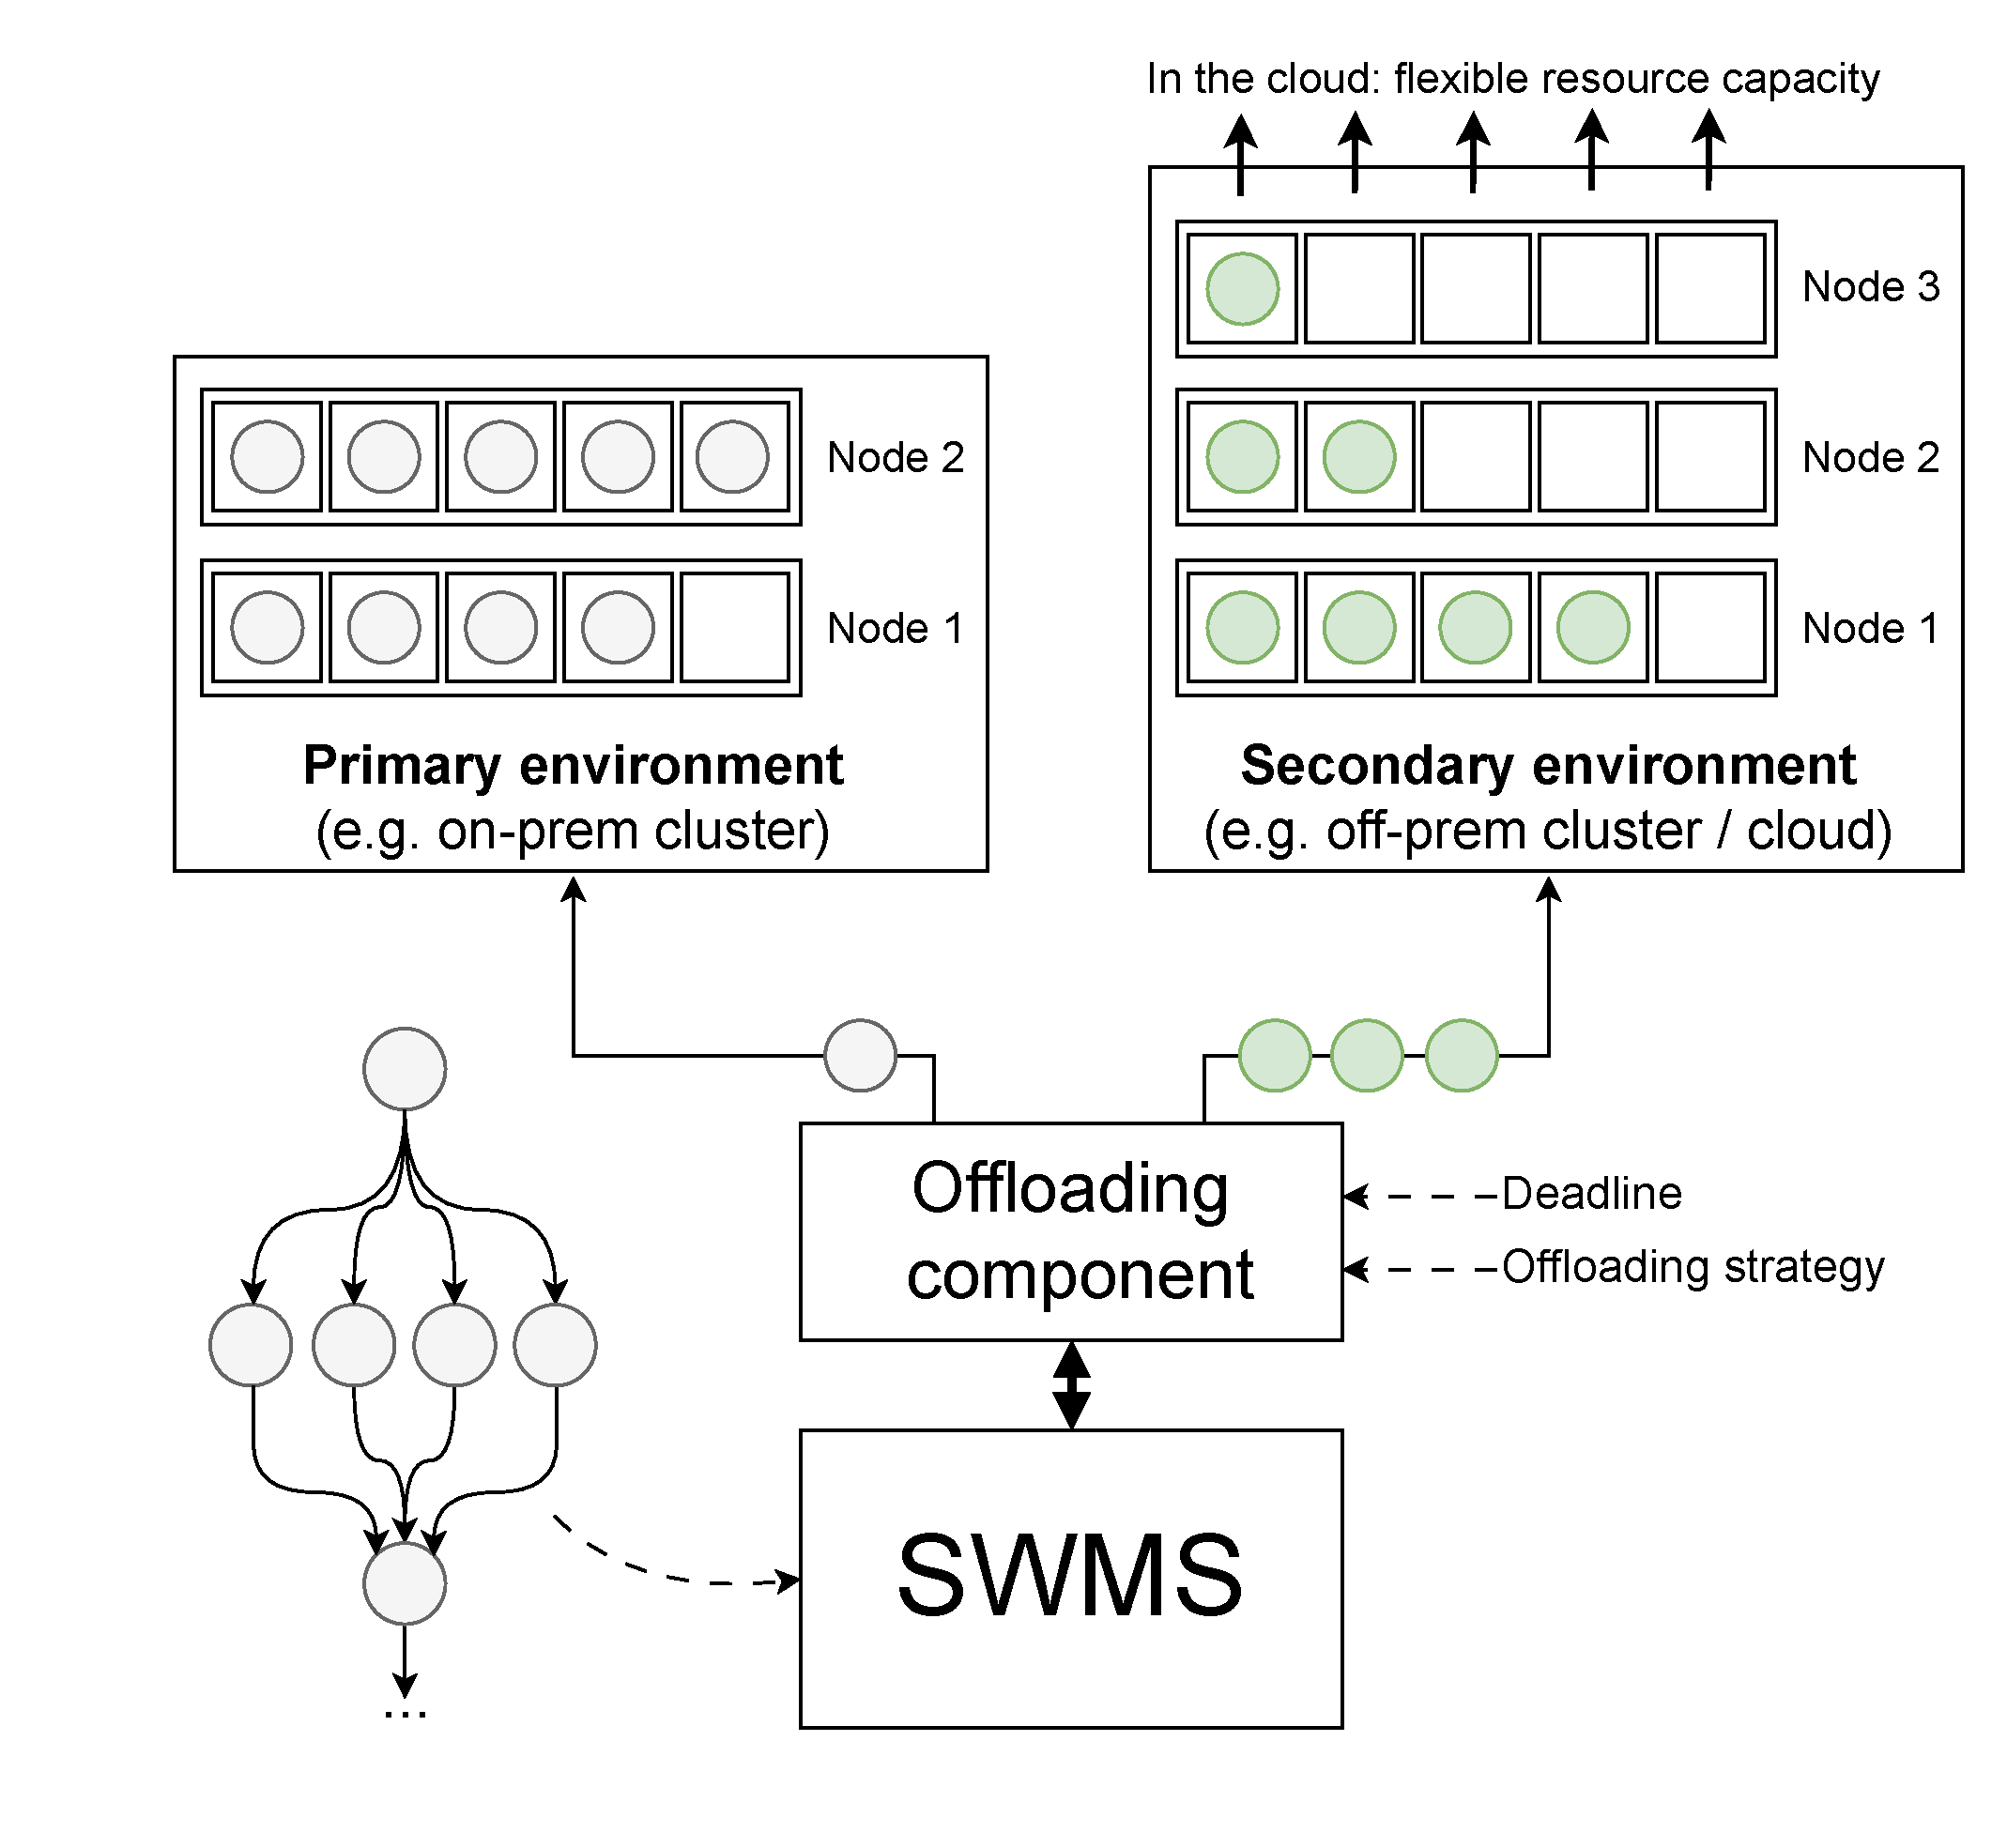
\includegraphics[width=1\linewidth]{./img/idea_introduction_smaller.drawio.pdf}
    \caption{Overview of the multi-cluster offloading problem for scientific workflows}
    \label{fig:intro}
\end{figure}

Fig.~\ref{fig:intro} illustrates the offloading scenario we consider in this paper. We assume a primary compute environment that serves as the default execution site, but may be unable to satisfy workflow deadlines due to limited resource capacity. To address this limitation, a secondary environment is available that can provide additional resources when necessary. 

All jobs are executed in the primary environment unless offloading is explicitly performed. A typical primary environment is an on-premise cluster that is readily accessible to users, provides limited computational capacity, and does not incur direct monetary cost. The secondary environment serves as an alternative execution site to which selected jobs can be offloaded. In practice, this secondary environment can correspond to an off-premise cluster with restricted capacity or to a cloud platform that offers resources on demand.

 As in many practical scenarios, particularly when using cloud resources, offloading introduces monetary costs proportional to the consumed resources and execution time. Therefore, the use of secondary environments must remain economically feasible, requiring careful control of offloading decisions. 

In this work, we propose the design and implementation of an offloading component that interacts with the SWMS to guide the workflow execution by determining which jobs should be offloaded to a secondary environment. This component is plugged into the SWMS and takes as input a user-defined deadline for the overall workflow makespan, as well as an offloading strategy \cite{ahmad_scientific_2021}.

The paper makes the following contributions:
\begin{enumerate}
  \item We propose a heuristic two-step approach: (i) predict job runtimes using linear models trained on historical data, and (ii) simulate workflow execution on multi-clusters using these predictions to select jobs for offloading that meet user-defined deadlines while minimizing cost.
  \item We provide our implementation as an extension to the Snakemake SWMS. The source code and the workflow execution data collected during our experiments are made publicly available.\footnote{{published after acceptance.}}
\end{enumerate}



\section{Problem Formulation}
\label{sec:problem}
As described in Section \ref{sec:introduction}, we intend to optimize the runtime of scientific workflows by offloading jobs to secondary clusters or the cloud. 

In a SWMS, a workflow is represented as a directed acyclic graph (DAG). A task denotes a logical step in the workflow DAG, while a job refers to a concrete execution instance of that task with specific inputs and outputs. 

The user sets a maximum allowed makespan (deadline) for the workflow. Executing jobs in the secondary execution environment incurs a monetary cost, while execution in the primary environment does not, as it corresponds to locally operated cluster infrastructure with fixed, pre-existing operational costs independent of individual workflow executions. 

The problem can be formulated as follows. 
\vspace{0.5em} 
Let: \begin{itemize} \item $J = \{j_1, j_2, \dots, j_n\}$ be the set of jobs of a scientific workflow. \item $J_{\text{off}} \subseteq J$ denote the subset of jobs that are offloaded to the secondary environment; the remaining jobs $J \setminus J_{\text{off}}$ are executed in the primary environment. \item $M(J_{\text{off}}) \in \mathbb{R}_{\geq 0}$ denote the makespan of the workflow when jobs in $J_{\text{off}}$ are offloaded. \item $D \in \mathbb{R}_{\geq 0}$ be the maximum allowed makespan (deadline). \item $C(J_{\text{off}}) \in \mathbb{R}_{\geq 0}$ denote the cost associated with offloading the jobs in $J_{\text{off}}$. \end{itemize} \vspace{0.7em} The goal is to find a subset of jobs $J_{\text{off}}^* \subseteq J$ such that: \[ M(J_{\text{off}}^*) \leq D \] \hspace{1em}and \[ J_{\text{off}}^* = \arg\min_{J_{\text{off}} \subseteq J,\ M(J_{\text{off}}) \leq D} C(J_{\text{off}}). \] \vspace{0.7em}

In other words, the objective of this constrained combinatorial optimization is to find a feasible offloading configuration that aims for completion within deadline $D$. Among all feasible configurations, the one with the lowest cost is sought. 

Additionally, we consider the following assumptions:

\begin{itemize}[label={}]
    \item (\textbf{A1}) Our runtime prediction approach does not yet account for differences in hardware configurations, thus we assume primary and secondary execution environments have identical or negligibly different hardware.
    \item (\textbf{A2}) We need historical execution traces with job runtimes and input sizes for model training.
    \item (\textbf{A3}) Workflow configuration parameters (for e.g. the algorithm a job uses) affecting runtime have remained constant.
\end{itemize}

\section{Approach}
\label{sec:approach}
This section presents our methodological framework, beginning with an overview of the heuristic design. Subsequently, we provide the algorithmic procedure of the heuristic and a description of the job selection mechanism for offloading.
\subsection{Overview\label{subsec:overview}} 

\begin{figure*}[t] \centering 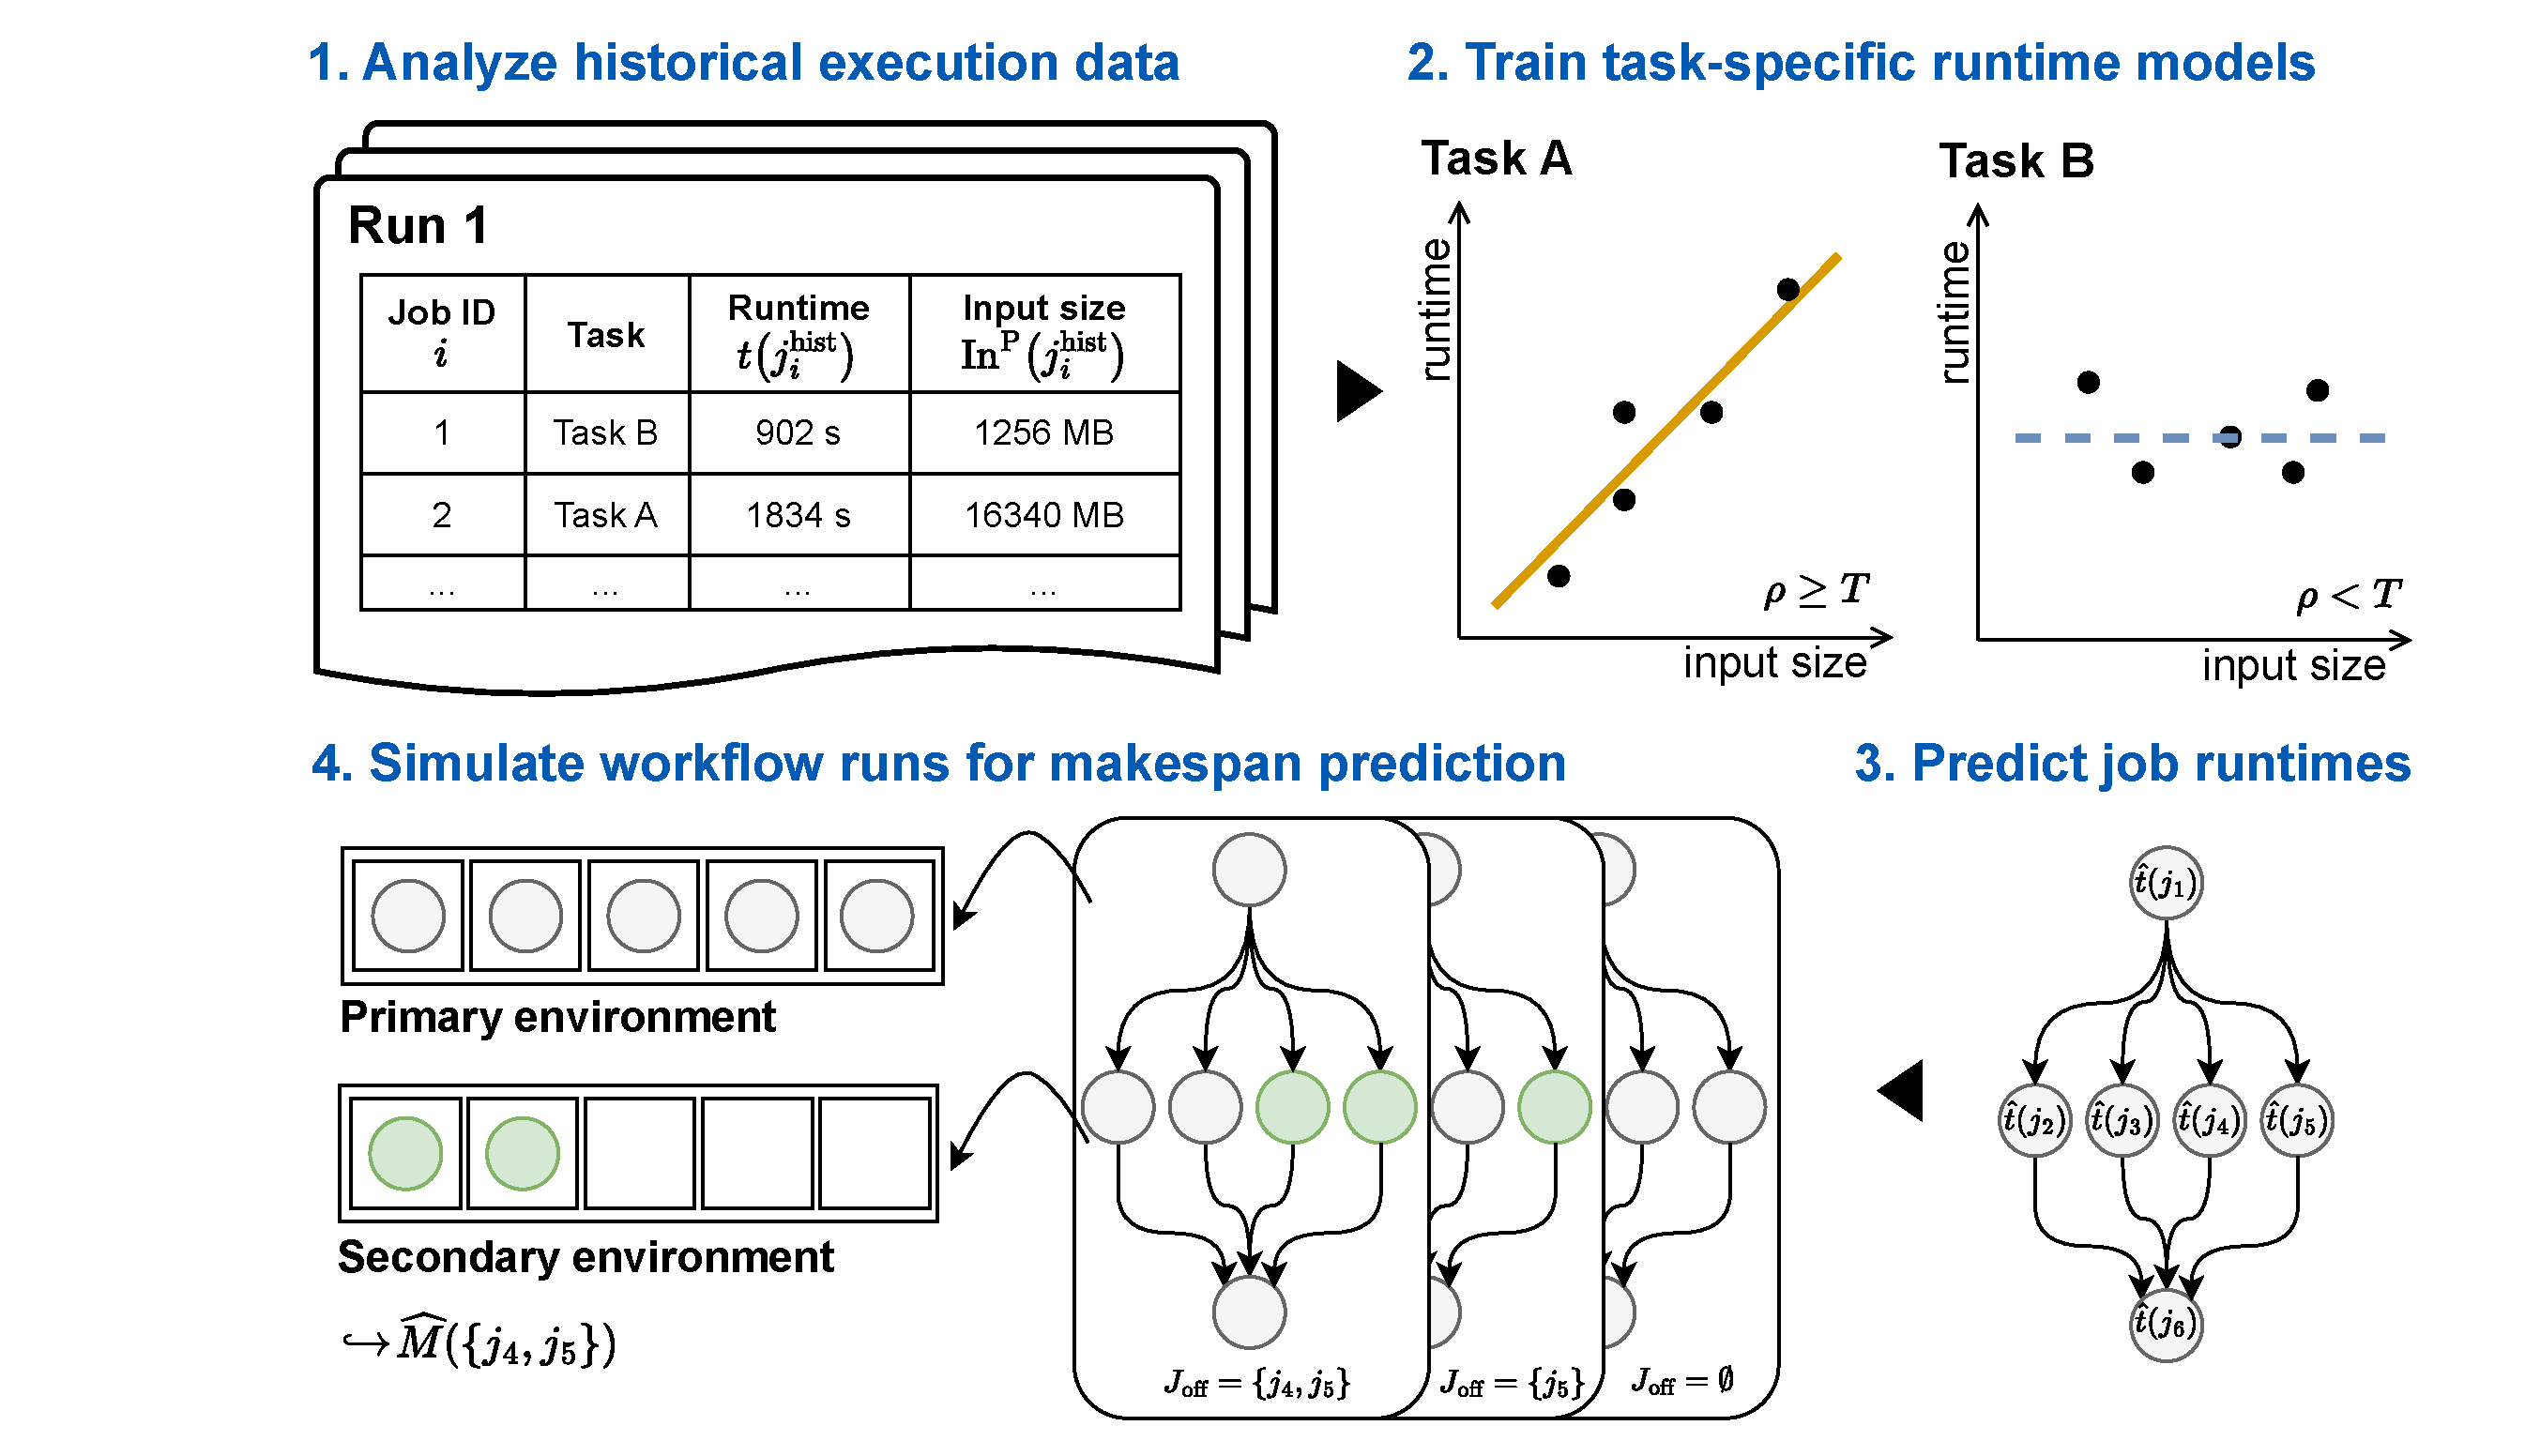
\includegraphics[width=0.8\linewidth]{./img/approach_overview.drawio.pdf} \caption{Overview of the multi-cluster makespan prediction approach} \label{fig:approach_overview} 
\end{figure*}

At a high level, our approach introduces makespan prediction to simulate job offloading under various selection criteria, thereby aiming at identifying offloading configurations that meet the user's requirement.
As a workflow is composed of a set of jobs $J$, its makespan is influenced by the runtimes $t(j)$ of these jobs $j \in J$, their dependencies, and the extent of job parallelization.
Since workflow makespan directly depends on job runtimes, we implement a two-step prediction approach:
We first predict the runtimes of all jobs in $J$ and then use these predictions to estimate the workflow makespan over the multi-cluster environment. 
Fig.~\ref{fig:approach_overview} illustrates the overview of the proposed multi-cluster prediction approach. Whereas phases 1 and 2 represent necessary pre-processing procedures, phases 3 and 4 together constitute the two-step predictive offloading framework.

\subsubsection{Phase 1}
In the first phase, we analyze the workflow execution, extracting all historical jobs $J^\text{hist} = \{j_1^\text{hist}, j_2^\text{hist}, \dots j_k^\text{hist}\}$, including their runtimes $t(j_i^\text{hist})$ and their primary input data sizes $\text{In}^\text{P}(j_i^\text{hist})$ (the sum over all input files). We also determine $\text{In}^\text{P-A}(j_i^\text{hist})$, defined as \[ \text{In}^\text{P-A}(j_i^\text{hist}) = \sum_{j \in \text{Anc}(j_i^\text{hist})} \text{In}^\text{P}(j) \] where $\text{Anc}(j_i^\text{hist})$ is the set of all ancestor jobs of $j_i^\text{hist}$. Determining $\text{Anc}(j_i^\text{hist})$ requires reconstructing the DAG of jobs for all workflow runs of the historical job records. In the following, we refer to the sum $\text{In}^\text{P}(j_i^\text{hist}) + \text{In}^\text{P-A}(j_i^\text{hist})$ as the \textit{combined primary input data size} of job $j_i^\text{hist}$.

\subsubsection{Phase 2}
 In the second phase, we train task-specific runtime models. 
 %The model training procedure takes inspiration from Bader et al. \cite{bader_lotaru_2024}, but relies on simple linear instead of Bayesian regression. 
 For each task, we consider all associated historical job records, independent of the workflow run. For a task with $k$ historical job records, this leaves us with a dataset $\mathcal{D}^\text{hist}$ of $k$ pairs of combined primary input data size and runtime: \[ \mathcal{D}^\text{hist}=\left\{\left(\text{In}^\text{P}(j_i^\text{hist}) + \text{In}^\text{P-A}(j_i^\text{hist}),\; t(j_i^\text{hist})\right)\right\}_{i=1}^{k}. \] 
 
 First, we check if a task's job runtimes scale linearly with their combined primary input data size. 
 %Bader et al. \cite{bader_lotaru_2024} demonstrated that runtime often correlates with input data size for bioinformatics tasks, but not for all such tasks. 
 In addition, even if a task's job runtimes correlate with input data size, they must not necessarily correlate with combined primary input data size.
 Accordingly, we compute the Pearson correlation coefficient $\rho$ for the data points in $\mathcal{D}^\text{hist}$. If $\rho \geq T$ for a threshold $T$, we assume linearity and train a linear regression model for that task with $\mathcal{D}^\text{hist}$ as training data. Then, for any job $j \in J$ derived from that task, the runtime prediction $\hat{t}(j)$ is given by: \[ \hat{t}(j) = \beta_{0} + \beta_{1} (\text{In}^\text{P}(j) + \text{In}^\text{P-A}(j)), \] where \( \beta_{0} \) and \( \beta_{1} \) are the task-specific regression coefficients. If $\rho < T$, the runtime prediction is instead defined as \[ \hat{t}(j) = \mathrm{median}\left\{ t\!\left(j_i^\text{hist}\right) \right\}_{i=1}^k. \]
 
\subsubsection{Phase 3 and 4}
In the third and fourth phase, we predict the runtimes $\hat{t}(j)$ of all jobs $j \in J$ and the resulting makespan of the workflow. To this end, we simulate workflow runs with varying $J_{\text{off}} \subseteq J$, predicting the particular makespan for each configuration. 

We intend to identify the optimal offloading configuration $J_{\text{off}}^*$ and its makespan prediction $\hat{M}(J_{\text{off}}^*)$. 
However, the naive approach of simulating all possible configurations $J_{\text{off}}$ is not feasible for large workflows, as the number of configurations grows exponentially with the number of jobs: There exist $|\mathcal{P}(J)|=2^{|J|}$ possible configurations $J_{\text{off}}$, where $\mathcal{P}(J)$ denotes the power set of $J$. Therefore, we propose a heuristic approach that iteratively selects jobs for offloading. The selection of jobs is based on an offloading strategy $\mathcal{S}$, which determines the order in which jobs are chosen and is discussed in detail in section \ref{par:makespan_prediction} and \ref{par:offloading-strategies}.


\subsection{Adaptive Multi-Cluster Offloading Heuristic}
\label{subsec:heuristic}
In this section, we provide a detailed description of how the results obtained in phase 3 (see Figure \ref{fig:approach_overview}) are utilized to perform makespan prediction in a multi-cluster environment (phase 4). Subsequently, these makespan predictions are then employed to determine the subset of jobs that should be offloaded.
The goal of our approach is that for a given $\mathcal{S}$, we compute the smallest set $J^{\mathcal{S}}_\text{off} \subseteq J$ such that $\hat{M}(J^{\mathcal{S}}_\text{off}) \leq D$. 
It is reasonable to assume that $J^{\mathcal{S}}_\text{off}$ is associated with the lowest cost out of all $J_{\text{off}} \subseteq J$ for $\mathcal{S}$ that meet the deadline, as the cost function strictly increases with the number of jobs (see Section~\ref{par:cost-estimation}). Finding $J_{\text{off}}^*$ is then equivalent to finding the offloading strategy $\mathcal{S}^*$ that minimizes $\hat{C}(J^{\mathcal{S}}_\text{off})$. This considerably reduces the search space, as only a subset of all possible offloading configurations is evaluated. At the same time, we might only find a local optimum, as the global optimum is not guaranteed to be within the search space.

% Prediction Aspect
\begin{algorithm}[h]
\label{lst:predict_workflow_makespan}
\caption{Workflow Makespan Prediction}
\SetKwInOut{Parameter}{Parameters}
\Parameter{\\
    \var{$D$} : Deadline (maximum makespan) \\
    \var{$\mathcal{S}$} : Offloading strategy \\
    }

\If{\var{$\mathcal{S}$} is deadline-aware}{
    \var{$J'_\text{off}$} $\gets$ $\emptyset$\;

    \var{$\hat{M}$}, \var{$J^{\mathcal{S}}_\text{off}$}, \var{$J_{\text{def}}$} $\gets$
    \func{simulateWorkflowRun}(\var{$\mathcal{S}$}, \var{$J'_\text{off}$})\;
    \While{\var{$\hat{M}$} $>$ \var{$D$}}{

        \If{\var{$J_{\text{def}}$} $\setminus$ \var{$J'_\text{off}$} $=$ $\emptyset$}{
            break\;
        }
        update \var{$J'_\text{off}$} by selecting job from \var{$J_{\text{def}}$} $\setminus$ \var{$J'_\text{off}$}\;
        \func{simulateWorkflowRun}(\var{$\mathcal{S}$}, \var{$J'_\text{off}$})\;
        update \var{$\hat{M}$} with \var{$\hat{M'}$} and \var{$J^{\mathcal{S}}_\text{off}$} with \var{$J'^{\mathcal{S}}_\text{off}$}\;
    }
}
\Else{
    \var{$\hat{M}$}, \var{$J^{\mathcal{S}}_\text{off}$}, \var{$J_{\text{def}}$} $\gets$
    \func{simulateWorkflowRun}(\var{$\mathcal{S}$}, None)\;
}

\Return \var{$\hat{M}$}, \var{$J^{\mathcal{S}}_\text{off}$}\;
\end{algorithm}
\paragraph{Multi-cluster Makespan Prediction under Offloading}\label{par:makespan_prediction}

The effective makespan $M(J_{\text{off}})$ and offloading cost $C(J_{\text{off}})$ of a workflow are only known after execution. Yet it is of great interest to find the optimal offloading configuration $J_{\text{off}}^*$ before execution, saving resources by avoiding expensive trial-and-error runs. 
Therefore we propose an approach to predict workflow makespan and associated offloading cost in advance.
We denote these predictions as $\hat{M}(J_{\text{off}})$ and $\hat{C}(J_{\text{off}})$. 

Algorithm~\ref{lst:predict_workflow_makespan} presents the heuristic more formally.
As parameters, it accepts a deadline $D$ and an offloading strategy $\mathcal{S}$.
It returns the predicted makespan $\hat{M}$, and the associated set of offloaded jobs $J^{\mathcal{S}}_\text{off}$. (For simplicity, we deviate slightly from the notation above, using $\hat{M}$ instead of $\hat{M}(J^{\mathcal{S}}_\text{off})$.) At different points, the algorithm calls the function \code{simulateWorkflowRun}. As input, this function accepts an offloading strategy and a set of jobs to be offloaded in the simulation and it returns $\hat{M'}$, $J'_\text{off}$ and $J_{\text{def}}$. 
%If the set is \code{None}, the offloaded jobs will be selected implicitly depending on the offloading strategy. %\code{simulateWorkflowRun} will be described in greater detail in Algorithm~\ref{lst:simulate_workflow_run}. It returns the predicted makespan $\hat{M'}$, the set of offloaded jobs $J'_\text{off}$ and the set of deferred jobs $J_{\text{def}}$. These are the jobs that had to be deferred at one point in the simulation, as they could not be executed immediately in one of the execution environments due to resource exhaustion.
The algorithm differentiates between deadline-aware strategies, which approach $D$ by iteratively simulating job selection until $D$ is met, and deadline-agnostic strategies, which do not consider any deadline (see Section~\ref{par:offloading-strategies} for details).
If $\mathcal{S}$ is deadline-agnostic (line 11), the algorithm simply calls the \code{simulateWorkflowRun} function once and returns the resulting makespan prediction and set of offloaded jobs.
If $\mathcal{S}$ is deadline-aware, the algorithm explicitly selects the jobs to be offloaded $J'_\text{off}$ and calls \code{simulateWorkflowRun} potentially many times.
With $\hat{M}'$, we denote the latest makespan prediction, and with $\hat{M}$, the best makespan prediction found so far.
Similarly, with $J'_\text{off}$, we denote the latest set of jobs selected for offloading, and with $J^{\mathcal{S}}_\text{off}$, the best set found so far, which is associated with $\hat{M}$.
In a first step, $J'_\text{off}$ is the empty set and the workflow is simulated once (lines 2-3).
If this results is a makespan prediction $\hat{M} \leq D$, the deadline can be met without offloading any jobs, and the algorithm returns.
Otherwise, the algorithm iteratively chooses additional jobs to be offloaded (lines 4-9).
In each iteration, as long as there is a job that has been deferred in the last simulation run and has not yet been offloaded (line 5), another job is added to $J'_\text{off}$ (line 7).
By restricting the selection to $J_{\text{def}} \setminus J'_\text{off}$, we ensure that only jobs that could not be executed in the primary environment are considered for offloading.
\begin{algorithm}[t]
\label{lst:simulate_workflow_run}
\caption{Workflow Run Simulation}
\SetKwInOut{Parameter}{Parameters}
\Parameter{\\
    \var{$\mathcal{S}$} : Offloading strategy \\
    \var{$J'_\text{off}$} : Set of jobs that must be offloaded
    }

\vspace{0.5em}

%Initialize \var{job\_queue}, \var{deferred\_jobs} as empty queues\;
%\vspace{0.2em}
%Initialize \var{time\_left\_per\_job} as empty map\;
%\vspace{0.2em}
Load \var{DAG}, \var{predictions}, \var{Q} and set \var{$\hat{M'}$} to 0\;
\vspace{0.5em}

\While{there are unfinished jobs in \var{DAG}}{
    \vspace{0.2em}
    add newly runnable \var{job} from \var{DAG} to \var{Q}\;
    %add newly runnable jobs $j \in \var{DAG}$ to \var{Q}\;
    \vspace{0.2em}
    \While{\var{Q} $\neq$ $\emptyset$}{
        \vspace{0.2em}
        %\var{job} $\gets$ \var{job\_queue}\func{.pop()}\;
        \vspace{0.2em}
        get \var{job} from \var{Q} and \func{assignJobToNode}(\var{job}, \var{$\mathcal{S}$}, \var{$J'_\text{off}$})\;
        %\var{node} $\gets$ \func{assignJobToNode}(\var{job}, \var{$\mathcal{S}$}, \var{$J'_\text{off}$})\;
        \vspace{0.2em}
        \If{\var{node} is found}{
            \vspace{0.2em}
           %\tcp{map job to runtime prediction}
            %\var{time\_left\_per\_job}[\var{job}] $\gets$ \var{predictions}[\var{job}]\; 
            \var{remaining\_job\_runtimes} $\gets$ runtime prediction \var{$\hat{t}$} for \var{job}\;
        }
        \vspace{0.2em}
        \Else{
            \vspace{0.2em}
            %\var{deferred\_jobs}\func{.push}(\var{job})\;
            store \var{job} and add to \var{Q} in next scheduling interval;
        }
    }
    %\vspace{0.2em}
    %\var{job\_queue}\func{.push}(\var{deferred\_jobs})\;
    %\vspace{0.2em}
    %\var{deferred\_jobs}\func{.clear()}\;
    %\vspace{0.2em}
    %\If{\var{time\_left\_per\_job} not empty}{
    \If{\var{remaining\_job\_runtimes} not empty}{
        \vspace{0.2em}
        %\var{time\_passed} $\gets$ min(\var{time\_left\_per\_job})\;
        \var{step\_time} $\gets$ min(\var{remaining\_job\_runtimes})\;
        update \var{$\hat{M'}$} by adding \var{step\_time}\;
        %\vspace{0.2em}
        %\var{$\hat{M'}$} $\gets$ \var{$\hat{M'}$} + \var{time\_passed}\;
        %\vspace{0.2em}
        %\var{newly\_finished\_job} $\gets$ argmin(\var{time\_left\_per\_job})\;
        %\vspace{0.2em}
        %\var{time\_left\_per\_job}.remove(\var{newly\_finished\_job})\;
        %\vspace{0.2em}
        \ForEach{\var{job} in \var{remaining\_job\_runtimes}}{
            \vspace{0.2em}
            %\var{time\_left\_per\_job}[\var{job}] $\gets$ \var{time\_left\_per\_job}[\var{job}] - \var{time\_passed}\;
            update each \var{job} by \var{step\_time}\;
        }
        \vspace{0.2em}
        reset resources of \var{node} that ran the latest \var{job} and remove from \var{DAG}\;
        %\vspace{0.2em}
        %mark \var{newly\_finished\_job} in \var{DAG} as finished\;
    }
}
\vspace{0.2em}
\Return \var{$\hat{M'}$}, all offloaded jobs, all jobs deferred at least once\;
\end{algorithm}
A job could be deferred even when offloaded if the secondary execution environment has insufficient resources. This case is most relevant for scenarios where the secondary environment is not a cloud environment with virtually unlimited resources, but another cluster.
The selection of the next offloaded job is based on $\mathcal{S}$.
Then, \code{simulateWorkflowRun} is called again with the updated set of offloaded jobs (line 8).
If the resulting makespan prediction $\hat{M}'$ is the best one found so far, $\hat{M}$ and $J^{\mathcal{S}}_\text{off}$ are updated (line 9).

If the secondary environment has insufficient resources, adding jobs to $J'_\text{off}$ does not necessarily lead to a smaller makespan prediction, as jobs could be deferred again.
In case there are no more deferred jobs that have not yet been offloaded, the algorithm aborts and returns the current $\hat{M}$ and $J^{\mathcal{S}}_\text{off}$ (lines 11-12).
This is because we assume that jobs should only be offloaded if they cannot be run in the primary execution environment due to resource exhaustion.
Given assumption A1 (Section~\ref{sec:problem}), we conclude that jobs running in the secondary environment would not finish earlier than in the primary environment, and therefore offloading them would not reduce the makespan but instead only increase the cost.
Although in that case the deadline cannot be met (line 6), $J^{\mathcal{S}}_\text{off}$ can still be considered the best-effort offload configuration.


% Simulation Aspect 
\paragraph{Simulation-based Offloading Optimization}
\begin{table}[t] 
\caption{Offloading strategies and their selection criteria} 
\centering 
\footnotesize 
\begin{tabular}{l|l} 
\textbf{Strategy} & \textbf{Description} \\ \hline  (1) PEFO & Offloads jobs when no primary resources are available  \\ (2) LJF & Offloads jobs with largest predicted runtime $\hat{t}(j)$ \\ (3) SISF & Offloads jobs with smallest primary input size $\text{In}^\text{P}(j_i^\text{hist})$
\end{tabular} 
\label{tab:offloading-strategies} 
\end{table} 
Given the above considerations, Algorithm~\ref{lst:simulate_workflow_run} represents the \code{simulateWorkflowRun} function invoked in Algorithm~\ref{lst:predict_workflow_makespan}.
As parameters, it accepts the offloading strategy $\mathcal{S}$ and the set of jobs to be offloaded $J'_\text{off}$.
The scheduling queue \code{Q} is processed until all jobs have been assigned to a node (line 5) or have been deferred because no node had sufficient resources (line 9).
The \code{assignToNode} function maintains an internal representation of simulated, available resources for each node in both cluster environments. If no node can provide sufficient resources, the function returns \code{None}, and the job is deferred.
The data structure \code{remaining\_job\_runtimes} serves to track the remaining runtime of running jobs, which at first is their runtime prediction (line 7).
Additionally it is ensured that, for deadline-aware strategies, a job is offloaded if and only if it belongs to $J'_\text{off}$, since the offloaded jobs have already been selected according to strategy $\mathcal{S}$. In the case deadline-unaware offloading, a job is only offloaded when the primary environment cannot meet its resource requirements at scheduling time and every job is assigned to the primary environment.
Once \code{Q} has been processed, deferred jobs are moved back into the queue to be retried in the next scheduling iteration. After each iteration, if there are running jobs, the job with the smallest remaining runtime is marked as finished. Its remaining runtime is added to the makespan and subtracted from the remaining runtimes of all other running jobs (lines 11-14), and the resources it used are released (line 15). In the next iteration, all jobs that become runnable due to this completion are added to \code{Q} and the loop continues until \code{Q} = $\emptyset$.

\paragraph{Offloading Strategies}\label{par:offloading-strategies}

Table \ref{tab:offloading-strategies} specifies the job selection criteria for offloading to a secondary environment. By comparing the results of Algorithm~\ref{lst:predict_workflow_makespan} between strategies, we select the strategy $\mathcal{S^*}$ with minimal offload cost $\hat{C}(J^{\mathcal{S^*}}_{\text{off}})=\hat{C}(J^{*}_{\text{off}})$. We consider both deadline-aware and deadline-agnostic strategies.

\begin{enumerate}

    \item \textbf{Primary Environment Fully Occupied (PEFO)} offloads a job exclusively when the primary environment does not possess sufficient resources to enable its immediate execution. PEFO serves as an offloading baseline, where the primary environment is constrained in capacity but otherwise unencumbered, whereas the secondary environment is associated with higher operational costs.
    \item \textbf{Longest Job First (LJF)} selects the job for offloading with the longest predicted runtime and is suited to settings where offloading incurs an additional overhead such as data transfer times or network latency, as long-running jobs are more likely to amortize such overhead. 
    \item \textbf{Smallest Input Size First (SISF)} selects jobs with the smallest combined primary input data size $\text{In}^\text{P}(j_i^\text{hist})$ and targets cases where offloading cost scales with input size. 
\end{enumerate}

To this end, these strategies are considered appropriate for the given configuration of task attributes, while additional selection criteria can be defined to account for specific job types or information regarding resource availability.

\paragraph{Workflow Cost Estimation}\label{par:cost-estimation}
% Makespan prediction yields For a given offloading configuration $J^{\mathcal{S}}_{\text{off}}$, we can predict the associated cost using the runtime predictions $\hat{t}(j_i)$ for $j_i \in J_{\text{off}}$.
For a given offloading configuration $J_{\text{off}}$, we model the cost prediction function $\hat{C}(J_{\text{off}})$ as a linear combination of job-level resource usages, weighted by unit cost factors:
\[
\hat{C}(J_{\text{off}}) = \sum_{j \in J_{\text{off}}} \hat{t}(j) \cdot \big(
\alpha_{\text{cpu}} \cdot \text{cpu}(j) +
\alpha_{\text{mem}} \cdot \text{mem}(j) +
\alpha_{\text{stor}} \cdot \text{stor}(j)
\big)
\]

Here, \(\hat{t}(j) \in \mathbb{R}_{\geq 0}\) denotes the predicted runtime of job \(j\) in hours, while \(\mathrm{cpu}(j)\), \(\mathrm{mem}(j)\), and \(\mathrm{stor}(j)\) denote the requested number of vCPUs, memory in GiB, and ephemeral storage in GiB, respectively. The coefficient \(\alpha\) corresponds to the unit price per resource in Table \ref{tab:unit-cost-factors}.

The values of these unit prices are based on the pricing of AWS Fargate (eu-central-1 region, Linux/X86 platform) as of 22 July 2025\footnote{\url{https://aws.amazon.com/fargate/pricing}}.
If jobs do not specify resource requests, we assume a default request of 1~vCPU, 2~GiB of memory and 20~GiB of ephemeral storage.

Thus, for any $J^{\mathcal{S}}_\text{off}$ found by Algorithm~\ref{lst:predict_workflow_makespan}, we can compute the associated cost prediction $\hat{C}(J^{\mathcal{S}}_\text{off})$ using the runtime predictions $\hat{t}(j)$ calculated earlier and the resource requests of each job.
In case a workflow definition does not specify resource requests for a job, we can fall back to default values (e.g., 1 vCPU, 2 GiB memory, 20 GiB storage).
%Note that the cost function does not model possible ingress or egress costs for transferring data to or from the secondary execution environment, which might be incurred by offerings of public cloud providers.

\begin{table}[t]
\caption{Unit cost factors used in the cost model}
\centering
\footnotesize
\setlength{\tabcolsep}{4pt}
\begin{tabular}{l|c|l}
\textbf{Resource} & \textbf{Unit Cost (\$)} & \textbf{Billing Basis} \\
\hline
CPU     & 0.04656  & per vCPU-hour \\
Memory  & 0.00511  & per GiB-hour \\
Storage & 0.000132 & per GiB-hour (ephemeral)
\end{tabular}
\label{tab:unit-cost-factors}
\end{table}




\section{Evaluation} 
\label{sec:evaluation}
We assess our method by determining how the different offloading strategies satisfy user-specified deadlines in a multi-cluster environment.

\subsection{Experimental Setup}\label{subsec:experimental-setup}

\begin{figure}[h]
    \centering
    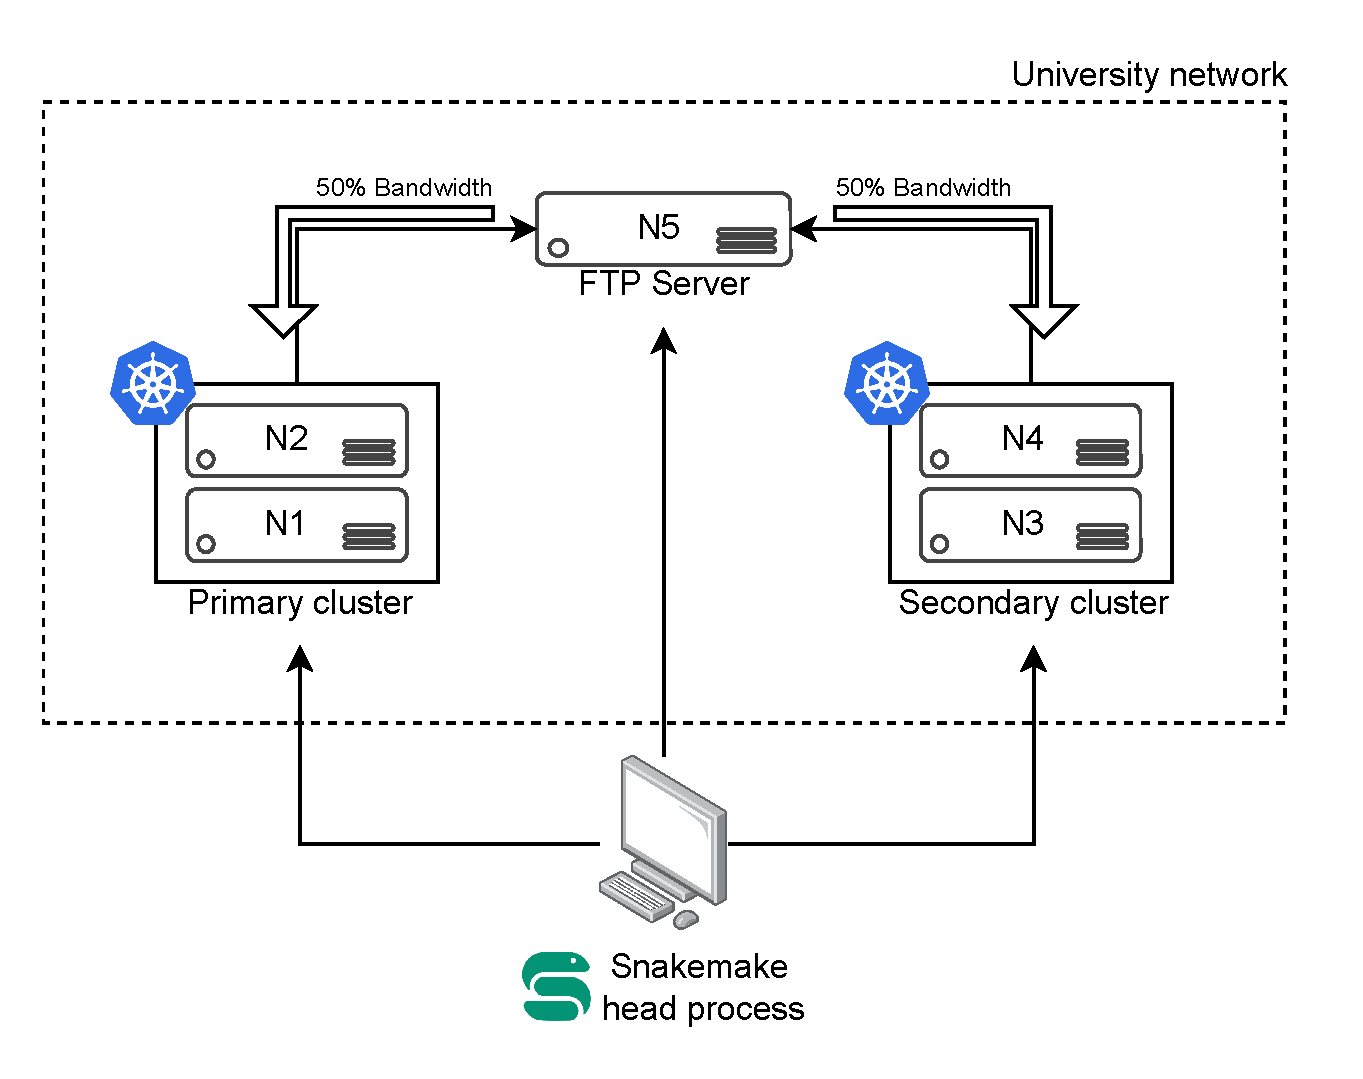
\includegraphics[width=1\linewidth]{./img/evaluation/experimental_setup.drawio.pdf}
    \caption{Kubernetes cluster setup for the experiments}
    \label{fig:experimental_setup}
\end{figure}

The following sections provide a description of the infrastructure configuration used for the evaluation, a brief account of the implementation of our approach, and an overview of the workflows used to assess our strategies.
\subsubsection{Infrastructure}
Fig.~\ref{fig:experimental_setup} shows the setup used for all experiments in this paper.
We employ two Kubernetes-based computing environments, referred to as the primary and secondary clusters. A Snakemake head process (version 9.5.1) runs on a local workstation with macOS 15.5 and connects, via a virtual private network (VPN), to two Kubernetes clusters that reside within the same university subnet. We use the tc utility\footnote{\url{https://linux.die.net/man/8/tc}} to allocate 50\% of the available bandwidth to the IP addresses of each Kubernetes cluster.
This is to keep FTP data transfer rates approximately constant between non-offloading and offloading scenarios.
Otherwise, when both clusters are in use and potentially twice as many jobs run concurrently, the available bandwidth per job would be halved, leading to significantly increased job runtimes.
Note that in scenarios where the load on the clusters is very different, data transfer rates may still vary significantly.
The head process submits all jobs to the clusters via our Offloading Plugin and Kubernetes Executor Plugin (Figure~\ref{fig:components_overview}). Each cluster has two Ubuntu~24.04 / Kubernetes~1.32.2 nodes (N1--N4), each with an AMD EPYC 7282 (16~cores, 32~threads, 2.8~GHz), 125~GiB RAM, 3.5~TB SSD, 10~Gbit/s Ethernet. A separate node N5 (Ubuntu~20.04, AMD EPYC 8224P, 24~cores, 48~threads, 2.55~GHz, 188~GiB RAM, 3.5~TB SSD, 10~Gbit/s) provides remote storage via FTP using the Snakemake FTP Storage Plugin.

% Build the bridge to the approach section and the algorithms.
\subsubsection{Implementation of Approach}\label{subsubsec:implementation}
All together, the Snakemake Offloading Utility (SOU), the offloading and the executor plugin implement our proposed approach in Section~\ref{sec:approach}. SOU provides a user interface to configure prediction parameters and offloading strategies and, from historical workflow data, estimates workflow makespan and execution costs. The Offloading Plugin mediates between Snakemake and executor plugins, dynamically switching between primary and secondary execution environments by forwarding execution calls for selected offloaded jobs. 
\begin{figure}[h]
    \centering
    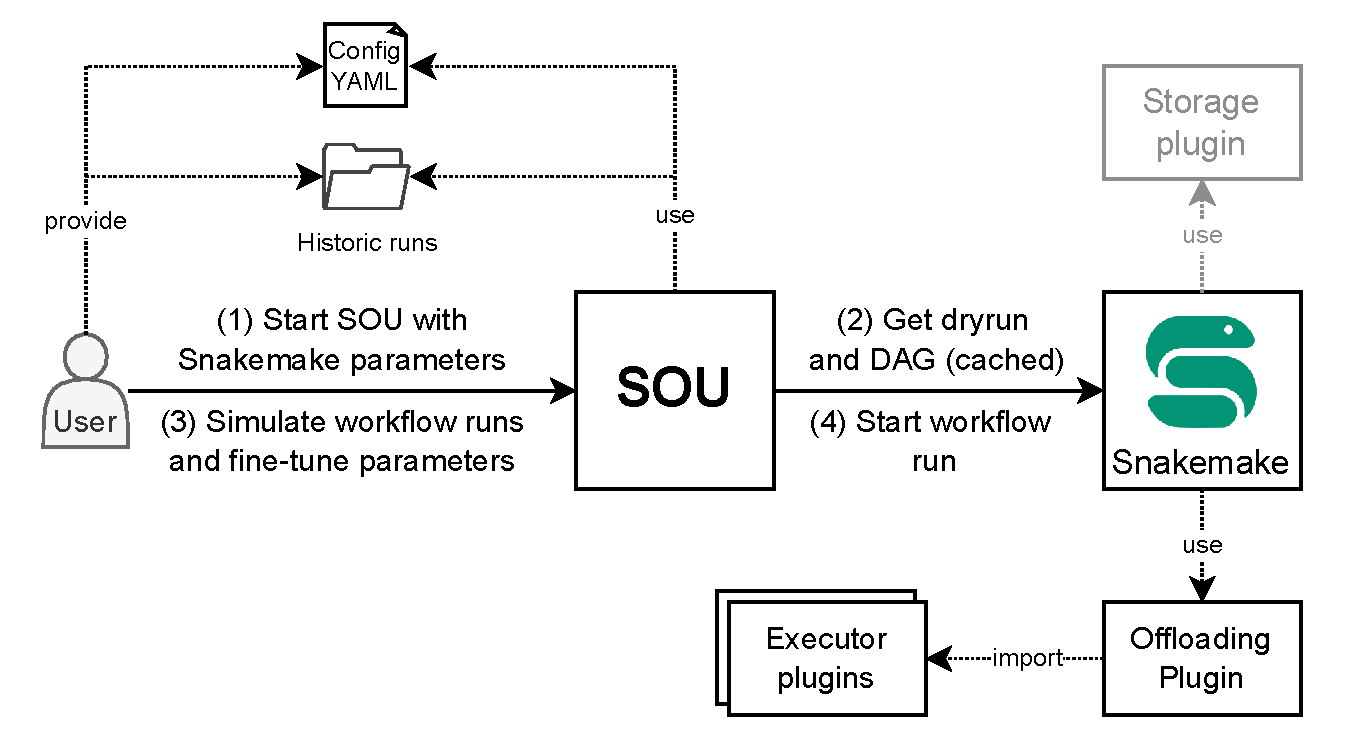
\includegraphics[width=1\linewidth]{./img/components_overview.drawio.pdf}
    \caption{Overview of offloading-related software components}
    \label{fig:components_overview}
\end{figure}
The Kubernetes executor plugin extends an existing Snakemake catalog package to integrate with the Offloading Plugin. 
To analyze the cost of the workflow, we set the cost factor parameters in the SOU configuration file to the values shown in Table~\ref{tab:unit-cost-factors} in Section~\ref{sec:approach}.

\subsubsection{Workflows and Experimental Data}
We evaluate our approach using the real-world bioinformatics workflows rna-seq-star-deseq2, stained-glass and dna-seq-varlociraptor from the Snakemake Workflow Catalog shown in Table~\ref{tab:workflow-comparison}.

These are among the 10 most popular workflows adhering to the catalog standards. They were selected to cover a variety of workflow characteristics, such as the number of tasks and jobs, the task dependency structure and the makespan.

\paragraph{rna-seq-star-deseq2}
The rna-seq-star-deseq2\footnote{\url{https://github.com/snakemake-workflows/rna-seq-star-deseq2}} workflow performs differential gene expression analysis on RNA sequencing data.
As input data, we use FASTQ files from the Genetic European Variation in Health and Disease (GEUVADIS) project \cite{the_geuvadis_consortium_reproducibility_2013, the_geuvadis_consortium_transcriptome_2013}.
The GEUVADIS project investigates the relationship between human genetic variation and gene expression.
In this context, high-depth RNA sequencing data from lymphoblastoid cell lines derived from 465 individuals has been generated.

\paragraph{stained-glass}
The stained-glass\footnote{\url{https://github.com/mrvollger/StainedGlass}} workflow creates identity heatmaps of genomic sequences.
This allows to visualize large-scale repetitive structures in genomes such as tandem repeats \cite{vollger_stainedglass_2022}.
As input data, we use a FASTA file of the human reference genome.
More specifically, we use the T2T-CHM13 v2.0 assembly, which is the first human genome assembly that includes all chromosomes (except Y) and telomeres \cite{nurk_complete_2022}.
In contrast to the other two workflows, where the number of input files is variable and influences the overall number of jobs, the stained-glass workflow depends only on a single FASTA file as input.
The overall number of jobs is determined by a workflow parameter that controls parallelization of the processing steps.
Still, we require multiple different input files for training and test data.
Therefore, we create input files with varying sizes from the T2T-CHM13 v2.0 assembly by extracting subsets of all available chromosomes with the samtools\footnote{\url{https://www.htslib.org}} suite.

\paragraph{dna-seq-varlociraptor}
The dna-seq-varlociraptor\footnote{\url{https://github.com/snakemake-workflows/dna-seq-varlociraptor}} workflow is an analysis pipeline for the detection and statistical evaluation of small variants (changes in  DNA sequence that involve a few nucleotides) and structural variants (changes involving bigger regions) from DNA sequencing data.
As input data, we use FASTQ files generated by Truong and Boeke \cite{truong_resetting_2017}.
The authors performed whole-genome sequencing on Saccharomyces cerevisiae strains which were humanized - that is, the core histones were replaced with their human counterparts.
Note that the task graph is not a DAG, as cycles can occur if jobs associated with the same task are executed at different stages of the workflow.

\subsection{Experimental Results}

We first train SOU’s makespan and cost predictors by running each workflow five times without offloading, using different input sizes to sample diverse task runtimes.

For evaluation, we run each workflow five more times on a separate fixed test dataset. As summarized in Table~\ref{tab:offloading-experiments}, we performed six experiments per workflow with varying offloading strategies and, when applicable, a chosen deadline per workflow. For the stained-glass workflow, we run only four experiments because LJF and SISF produce identical offloading configurations given their DAG structure. 

Table~\ref{tab:prediction-results} constitutes the principal reference for the presentation of our results. It reports a comparison between the observed median makespan, the predicted makespan, and the number of offloaded jobs, together with the associated costs incurred in the secondary environment. %As evaluation metrics, we employ the normalized deadline adherence score, the mean prediction error and costs in \$. 
The predicted error (PE) shown for the makespan and cost is calculated as follows:
\vspace{0.3em}
\[
\text{PE} = \frac{\text{predicted\_value} - \text{median}(\text{observed\_values})}{\text{median}(\text{observed\_values})}
\]

%\subsubsection{Deadline Adherence\label{subsubsec:deadline-adherence}}
\begin{table}[t]
\caption{Number of tasks and jobs per workflow}
\centering
\footnotesize
\setlength{\tabcolsep}{4pt}
\begin{tabular}{l|ccc}
\textbf{Workflow} & \textbf{\# Tasks} & \textbf{\# Jobs} \\
\hline
a) rna-seq-star-deseq2   & 16 & 135  \\
b) stained-glass         & 10 & 44   \\
c) dna-seq-varlociraptor & 40 & 744 
\end{tabular}
\label{tab:workflow-comparison}
\end{table}

% Figure Makespan and Offloading Dependence
\begin{figure*}[t]
  \centering
  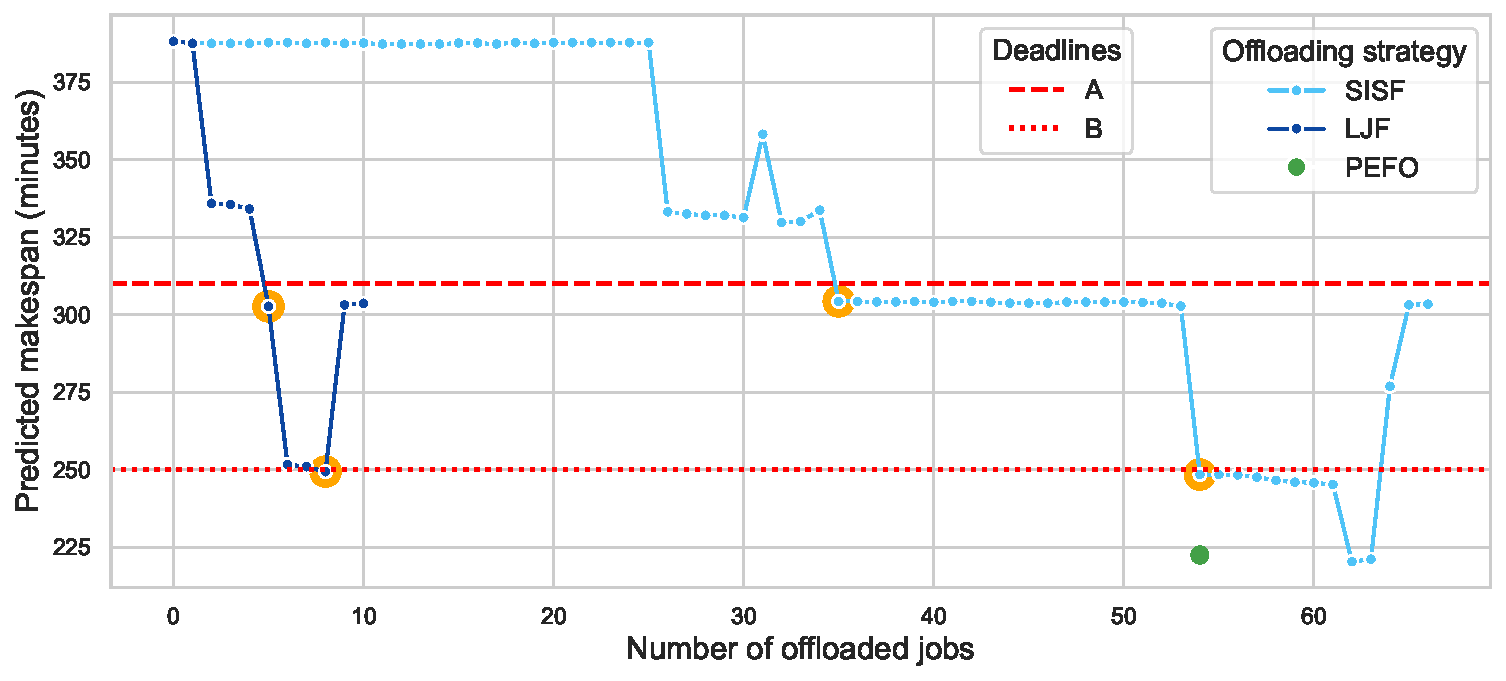
\includegraphics[width=0.8\linewidth]{img/evaluation/workflow_offloading_steps_rna-seq-star-deseq2.pdf}
  \caption{Dependence of workflow makespan prediction on the number of offloaded jobs for rna-seq-star-deseq2}
  \label{fig:makespan-offloading-dependence}
\end{figure*}

% Text on the figure, how it behaves, etc.
Figure~\ref{fig:makespan-offloading-dependence} shows the makespan predictions recorded in each simulation run during the iterative job selection of LJF and SISF (Algorithm~\ref{lst:predict_workflow_makespan}), using the rna-seq-star-deseq2 workflow as an example. The orange points mark the offloading configurations chosen by SOU for the deadlines, corresponding to Table~\ref{tab:prediction-results}. SOU selects the configuration with the fewest offloaded jobs that still meets the deadline. Workflow deadlines were chosen to produce clearly distinct makespan predictions. For comparison, the PEFO makespan prediction is also shown. 

\subsubsection{Dependency between Offloaded Jobs and Makespan Prediction}

\begin{table}[t]
% \small
\caption{Overview of the offloading experiments}
\centering
\begin{tabular}{r|cc}
\textbf{Exp.} & \multicolumn{1}{l}{\textbf{Offl. strategy}} & \multicolumn{1}{l}{\textbf{Deadline}} \\
\hline
1                   & None                                        & N/A                                   \\
2                   & PEFO                                        & N/A                                   \\
3                   & LJF                                         & A                                     \\
4                   & LJF                                         & B                                     \\
5                   & SISF                                        & A                                     \\
6                   & SISF                                        & B                                    
\end{tabular}
\label{tab:offloading-experiments}
\end{table}

In particular, the predicted makespan for SISF remains approximately constant for offloading levels between 0 and 25 jobs. This behavior indicates that, within this range, our heuristic predominantly favors LJF over SISF, because LJF is able to satisfy the deadline constraint after offloading only 6 jobs, in contrast to SISF, which requires the offloading of 35 jobs to meet the same deadline. This behavior is consistent with the objective of minimizing the number of offloaded jobs to still meet the deadline and, consequently, the total execution cost. Therefore, the intuitive expectation that monetary costs increase with a higher number of offloaded jobs while makespan decreases is generally confirmed. This pattern is substantiated by the data in Table~\ref{tab:prediction-results}, which exhibit strong negative Pearson correlation coefficients for makespan and incurring cost ($\rho = -0.925$, $-0.997$, and $-0.845$ for rna-seq-star-deseq2, stained-glass, and dna-seq-varlociraptor, respectively). However, Fig.~\ref{fig:makespan-offloading-dependence} also shows that, for the SISF strategy, the offloading of additional jobs (after 31 and 65 jobs) increases the predicted makespan. In Section~\ref{sec:discussion}, we analyze this behavior and discuss possible reasons for these findings.

\subsubsection{Workflow Makespan Prediction without a Deadline\label{subsubsec:offloading-without-deadline}}
Experiments 1 and 2 compare inactive offloading with offloading guided by the PEFO strategy.
Across all workflows, PEFO reduces median makespans vs inactive offloading by 130~min 28~s (-36.51\%) for rna-seq-star-deseq2, 25~min 16~s (-30.99\%) for stained-glass and 54~min 29~s (-26.07\%) for dna-seq-varlociraptor. Absolute prediction errors range between 1.94\% for rna-seq-star-deseq2 and 12.76\% for dna-seq-varlociraptor. Only rna-seq-star-deseq2 with inactive offloading exceeds the median makespan by 8.63\%.

\subsubsection{Workflow Makespan Prediction with a Deadline \label{subsubsec:offloading-with-deadline}}
To evaluate experiments 3-6 based on Table~\ref{tab:prediction-results}, we compare the LJF and SISF strategies with two different deadlines each.
% General performance
Considering only experiments where the deadline is satisfied by our method, workflows rna-seq-star-deseq2 and stained-glass meet their deadlines with an average slack of approximately 15 minutes. In contrast, dna-seq-varlociraptor consistently violates its deadlines, exceeding them by an average of about 8 minutes.
Deviations in the median makespan from the predicted makespan range from 9 seconds to 35 minutes (PE -0.21\% - 16.88\%).
In particular, the largest prediction errors do not occur between workflows. Instead, they appear only for the SISF strategy in the rna-seq-start-deseq2 workflow (PE 10.66\% \& 16.88\%). 

For rna-seq-star-deseq2, the makespan is generally overestimated. It is slightly underestimated only for LJF under deadline B with a PE of -2.48\%. Prediction errors range from -2.48\% (LJF, B) to 16.88\% (SISF, B). Deadline A is satisfied by both offloading strategies, whereas deadline B is met only by SISF. Although the predicted makespans are similar, SISF produces a substantially lower median makespan than LJF for both deadlines, at the cost of higher prediction errors (10.66\%, 16.88\% vs. -2.48\%, 2.80\%).

For stained-glass workload, the makespan is consistently underestimated with relative errors of -0.21\% (A) and -2.32\% (B), while both deadlines are nevertheless met. 

For dna-seq-varlociraptor, the makespan is systematically underestimated, with prediction errors ranging from \(-7.84\%\) (SISF/B) to \(-4.40\%\) (LJF/A). In none of the experiments are the specified deadlines met, as the actual makespan exceeds the deadline by an average of 10 minutes. The LJF scheduling strategy yields a lower median makespan than SISF for both deadline configurations.

\subsubsection{Offloading Costs}

The resulting offloading costs, summarized in Table~\ref{tab:prediction-results}, reveal that the LJF and SISF strategies, although producing higher makespans, still achieve lower overall costs than the naive offloading baseline (PEFO). This highlights a key trade-off between, on the one hand, minimizing execution time by fully utilizing and saturating local compute resources before offloading, and, on the other hand, deliberately satisfying a given deadline while selecting the cost-optimal configuration.
To illustrate the magnitude of improvement achievable within a single workflow, we consider rna-seq-star-deseq2, which exhibits the largest cost differences between strategies. Under PEFO, this workflow incurs a median cost of \$5.151 with a median makespan of 226.90 minutes, whereas the lowest-cost deadline-aware configuration (LJF with a 310-minute deadline) reduces the median cost to \$2.065 while achieving a comparable median makespan of 294.43 minutes. Similar behavior can be observed for dna-seq-varlociraptor, where costs decrease from \$4.097 under PEFO to \$0.708 with LJF and \$1.449 with SISF. In total, deadline-aware strategies achieve an average cost reduction of 52\% compared to PEFO, corresponding to a geometric mean cost factor of 0.48, calculated by forming per-experiment cost ratios (LJF and SISF relative to PEFO) using median observed costs and aggregating these ratios across all applicable workflows and experiments. These examples show that substantial cost reductions can be achieved within the same workflow, even when allowing for moderate increases in makespan.

\begin{table*}[t]
\caption{Makespan and cost prediction results across workflows}
\centering
\footnotesize
\setlength{\tabcolsep}{4pt}
\begin{tabular}{l|l|rrrrrr}
\textbf{Workflow} & \diagbox{\textbf{Metric}}{\textbf{Experiment}}
& \textbf{1} & \textbf{2} & \textbf{3} & \textbf{4} & \textbf{5} & \textbf{6} \\
\cline{3-8}
 &  & \multicolumn{6}{c}{\textbf{Offloading Strategy}} \\
 &  & None & PEFO & LJF & LJF & SISF & SISF \\
\hline
rna-seq-star-deseq2
 & \# Offloaded jobs          & 0 & 27 & 5 & 8 & 35 & 54 \\
 & Pred. Makespan (min)       & 388.20 & 222.50 & 302.67 & 249.37 & 304.27 & 248.45 \\
 & Median Makespan (min)      & 357.37 & 226.90 & 294.43 & 255.70 & 274.97 & 212.57 \\
 & PE Makespan (\%)           & 8.63 & -1.94 & 2.80 & -2.48 & 10.66 & 16.88 \\
 & Deadline (min)             & N/A & N/A & 310 & 250 & 310 & 250 \\
 & Median Cost (\$)           & 0 & 5.151 & 2.065 & 3.805 & 1.715 & 4.831 \\
\hline
stained-glass
 & \# Offloaded jobs          & 0 & 8 & 2 & 6 & N/A & N/A \\
 & Pred. Makespan (min)       & 78.38 & 53.53 & 72.17 & 59.74 & N/A & N/A \\
 & Median Makespan (min)      & 81.53 & 56.27 & 72.32 & 61.17 & N/A & N/A \\
 & PE Makespan (\%)           & -3.87 & -4.86 & -0.21 & -2.32 & N/A & N/A \\
 & Deadline (min)             & N/A & N/A & 75 & 65 & N/A & N/A \\
 & Median Cost (\$)           & 0 & 0.736 & 0.218 & 0.586 & N/A & N/A \\
\hline
dna-seq-varlociraptor
 & \# Offloaded jobs          & 0 & 279 & 28 & 47 & 232 & 325 \\
 & Pred. Makespan (min)       & 199.46 & 134.80 & 173.72 & 159.34 & 178.73 & 159.90 \\
 & Median Makespan (min)      & 209.00 & 154.52 & 181.72 & 168.98 & 187.42 & 173.52 \\
 & PE Makespan (\%)           & -4.56 & -12.76 & -4.40 & -5.70 & -4.64 & -7.84 \\
 & Deadline (min)             & N/A & N/A & 180 & 160 & 180 & 160 \\
 & Median Cost (\$)           & 0 & 4.097 & 0.708 & 1.941 & 1.449 & 2.654 \\
\end{tabular}
\label{tab:prediction-results}
\end{table*}

\section{Discussion}
\label{sec:discussion}
From the experimental results, we can overall derive that PEFO, LJF and SISF substantially reduce workflow makespan versus inactive offloading. Our heuristic is effective in identifying a minimal subset of jobs for offloading, thereby reducing execution costs while still meeting the prescribed deadline constraint. 

However, we generally observe that some deadlines are met by a substantial margin, whereas others are missed by only a small deviation. These slight discrepancies between the median observed makespan and the predicted, deadline-compliant makespan motivate a more detailed examination.

For the LJF and SISF strategies, we observe from Fig.~\ref{fig:makespan-offloading-dependence}, that the predicted makespan does not necessarily exhibit a monotonic decrease as the number of offloaded jobs increases. We conclude that excessive offloading does not necessarily reduce the predicted makespan and can instead lead to performance degradation that eventually violates the deadlines. This occurs because the simulation ignores resource constraints in the secondary environment, so over-offloading causes contention and delayed execution, potentially increasing the makespan. This effect is not expected to occur in settings where the secondary environment is a public cloud, as these typically offer virtually unlimited resources.
However, in our experimental setup resources are limited, and we see that deadlines are not always met due to prediction errors. As can be observed in Table~\ref{tab:prediction-results}, this is especially the case when the makespan prediction for a given deadline is very close to the deadline itself. In this regard, deadlines can be interpreted as soft constraints. SOU does not guarantee that the selected offloading configuration will meet the deadline, but rather tries to find an offloading configuration that is predicted to meet it. 
There are several possible explanations for the observed prediction errors.

Firstly, as part of the two-stage prediction approach, workflow makespan prediction is based on job runtime predictions, which are inherently uncertain. The prediction error of job runtimes can negatively affect the workflow simulation, leading to larger errors in makespan prediction. 
% Reasons for inaccurate runtime predictions
When multiple jobs of a task have to share the resources of the execution environment with many other jobs, contention occurs. This can lead to increased variability in job runtimes, since competing jobs may affect each other's performance, thus significantly contributing to the prediction errors. Additionally, runtime prediction makes use of combined primary
input data of jobs. If a job has no primary input data of its own, model training relies completely on the primary input data of its ancestors. In some cases, the input data of the primary ancestor is identical for all historical jobs of a certain task, making it impossible to calculate the Pearson correlation coefficient. In effect, the median of historical runtimes is used as a fallback, eventually making job runtime predictions inaccurate. 

Secondly, if offloading is active, the simulation is sensitive to small deviations in job runtimes. For example, if a job is predicted to run slightly longer than it actually does, it may be selected for offloading during the simulation, even if there are sufficient resources available in the primary environment during the actual workflow run. 

Lastly, the simulation does not account for potential job errors. If a job fails during the actual workflow run, it is retried, provided retrying is enabled in the workflow configuration. (The maximum number of retries was set to 5 for all workflows used in the experiments.) This can lead to an increase in makespan compared to the simulation, which assumes that all jobs are completed successfully on the first attempt. 





\section{Related Work}
\label{sec:relatedwork}
This Section reviews scientific literature related to this paper.
We focus on two main areas: runtime prediction of scientific workflow jobs and offloading of jobs, in particular within heterogeneous distributed computing environments.

\subsection{Job Runtime Prediction}
Many approaches for runtime prediction of scientific workflow jobs have been proposed, varying in model type and complexity, features selected, and whether they rely on offline training or online updates.

Da Silva et al. \cite{da_silva_online_2015} estimate job runtime and resource usage based on the size of the input data. The method uses historical data to identify correlations between input size and job parameters (including runtime), and continuously updates models during workflow execution. If no clear correlation is found, a density-based clustering algorithm partitions the profiling data to isolate consistent subsets with more predictable behavior.

Hilman et al. \cite{hilman_task_2018} propose an online incremental learning approach for adapting performance variability in cloud-based multi-tenant Workflow as a Service platforms. They lower the runtime prediction error by continuously updating the online incremental model with new execution data, leveraging time-series monitoring data (CPU, memory, I/O) and features extracted via time-reversal asymmetry statistics.

The work by Bader et al. \cite{bader_lotaru_2024, bader_lotaru_2022} focuses on improving the absolute prediction error and predict workflow job runtime on heterogeneous clusters without relying on historical data. They profile node microbenchmarks (CPU, memory, and I/O) and then execute locally on downsampled input data to obtain job-specific metrics such as input size and runtime. Using these metrics, the method models the relationship between input size and runtime, providing prediction uncertainty estimates useful for scheduling.

Balis et al. \cite{balis_evaluation_2023,balis_improving_2024} investigate and conduct an empirical evaluation of ML-based runtime prediction for scientific workflow jobs, concluding that two-stage pipelines for job runtime prediction generally improve accuracy. In the first stage, intermediate job parameters (e.g., mean CPU usage, used memory, total read bytes) are predicted and then used as features in the second stage to predict job runtime. 


\subsection{Job Offloading}
Various approaches for workflow job offloading have been proposed, particularly in fog and mobile cloud computing. 

In mobile cloud computing, Zhang et al. \cite{zhang_task_2017} investigate offloading for scientific workflows in Mobile Cloud Computing, where resource-constrained smart mobile devices (SMDs) use cloud infrastructures for computation- and data-intensive jobs. They define a cost model for VM utilization in Infrastructure as a Service clouds and propose a genetic algorithm on SMDs to map workflow jobs between cloud VMs and SMDs. Standard genetic operators (encoding, crossover, mutation, population initialization) are adapted to workflow offloading, and data placement constraints (e.g., due to privacy) are handled by enforcing local execution of affected jobs. Thus achieving near-optimal monetary cost and SMD energy consumption while satisfying deadline and data placement constraints. 

Similarly, Wang et al. \cite{wang_energy-efficient_2019} address mobile device energy consumption with a deadline-aware job offloading strategy for mobile cloud workflows. Their decision model selects local execution or cloud offloading based on job characteristics (e.g., transmission data size, workload) and the dynamic wireless channel state, whose fluctuations strongly affect offloading energy efficiency.

Shukla et al. \cite{shukla_fat-eto_2023} propose FAT-ETO, a rank-based task offloading algorithm for heterogeneous fog–cloud environments that integrates fuzzy logic with multi-criteria decision-making. By ranking edge devices, fog nodes, and cloud nodes for each workflow job based on weighted decision criteria, they show that FAT-ETO reduces makespan and energy consumption compared to existing heuristics, at the expense of slightly higher cost, particularly effective for workflows with many jobs. 

Kaur et al. \cite{kaur_focalb_2021}, introduce FOCALB, a fog computing–based architectural model and load-balancing framework designed to offload scientific workflow jobs across fog–cloud infrastructures. In contrast to FAT-ETO, FOCALB assumes that workflow jobs are submitted from user endpoint devices and executed only on fog nodes and cloud servers. With hierarchical scheduling, jobs are first assigned to nearby fog nodes to reduce network overhead, and the utilization layer is continuously monitored. When resource capacity limits are exceeded, and deadlines permit, jobs are selectively offloaded to cloud servers. A dedicated load-balancing module redistributes jobs among fog nodes within a cluster to ensure fair reutilization and avoid overload condition, thus optimizing both makespan and energy consumption.


\section{Conclusion}
\label{sec:conc}
In this paper, we propose a method that offloads scientific workflow jobs between multi-cluster environments to meet user-defined deadlines.
To this end, we use historical data to train regression models that predict job runtimes from input size and then simulate DAG execution to estimate makespan and cost for two deadline-aware and one deadline-agnostic offloading strategies.
We implemented our method in Snakemake and evaluated it on three real bioinformatic workflows in Kubernetes clusters. 
The results show reduced makespans of up to 36.51\% compared to single-cluster executions and makespan prediction errors ranging from 0.21 to 16.88\%. On average, makespan deadlines are met with an average margin of 14 minutes, while achieving cost reductions of approximately 52\% compared to naive offloading.

While we demonstrated the feasibility of our method, future work should focus on reducing the prediction errors caused by uncertainties during runtime.
By incorporating richer execution-state features and employing non-linear, online learning models, we plan to alleviate this limitation and facilitate dynamic, runtime re-evaluation of offloading decisions \cite{da_silva_online_2015, hilman_task_2018} to guaranty deadline constraints. 
To account for heterogeneous execution environments, we plan to extend our predictions with the approach of Bader~et~al.~\cite{bader_lotaru_2022, bader_lotaru_2024}. 
Further refinements of the offloading criterion could target adverse operating conditions such as high network latency and include power and CO\textsubscript{2} metrics to enable environmentally sustainable multi-cluster offloading.





\section*{Acknowledgments}
%\thanks{Funded by the Deutsche Forschungsgemeinschaft (DFG, German Research Foundation) as FONDA (Project 414984028, SFB 1404).}
\thanks{The acknowledgments are omitted for double-blind submission.}


\bibliographystyle{IEEEtran}
\bibliography{bibliography}



\end{document}
